% ======================================================
% Compile: xelatex 5state_powerlaw_hd.tex
% Path:    reference/eq17_analysis/derivation/5state_powerlaw_hd.tex
% Purpose: Full-detail derivation of the 5-state POWER-LAW-gain eq17 controller
%          + closed-loop EKF, following the section-by-section flow of the baseline
%          RevisedConrol_Vpersonal.pdf, and mirroring 6state_curvature_hd.tex, but
%          REPLACING the Taylor gain hierarchy [a_h, a'_hd, delta_a'_hd] with a
%          reduced two-parameter gain law with sub-state [a_h, p] (gain level +
%          exponent), whose slope obeys
%              a_h' = (1/R)(p/(h_bar-1)) a_h(a_o-a_h)/a_o.
%          The far-field gain a_o = a_nom = a_h(h_bar->inf); c and its amplitude K
%          never enter the recursion (a_h's level carries them), so they are dropped.
%          h-notation, h_bar = h/R (radius R threaded through
%          every d/dh = (1/R) d/dh_bar and Dh_d = R * Dh_bar_d interface).
%          State x = [ dh1, dh2, dh3, a_h, p ].  Scope: ends at the boxed 5x5 F_e
%          (Q/R left as symbols, as in the baseline).
% Style mirrors 6state_curvature_hd / 5state_derivation (monochrome, \fbox on key
% results, run-in bold-underline \hd headings).
% ---- BUILD STATUS: Stage E COMPLETE (sections 1-13; F_e + Q + R). Q Path C strict:
%      Q33=4kBT a_h, Q44=a_h'^2 Q33, Q34=-a_h' Q33, Q55=0 (rank-1 gain block; MA-tail
%      inflation -> closed-loop variance, not Q). R1=sig_nh^2; R2=a_cov*IF_var*(a_h+xi)^2
%      (ported IIR chi-sq readout, C_dpmr=2+1/(1-lc^2), C_n=2/(1+lc), xi=(C_n/C_dpmr)
%      sig_nh^2/(4kBT)); curvature-Jensen bias + d-step q4 accumulation deferred.
% ---- (earlier) Stage D (sections 1-11; ends at boxed 5x5 F_e). A: motion
%      error -> delta_h[k+1] = lc*delta_h - F_dh*e_ah - eps_h. B: gain sub-state [a_h, p],
%      slope a_h' = s_h[k]/R, s_h[k] := da_h/dh_bar = (p/(h_bar-1)) a_h(a_o-a_h)/a_o
%      (R-free, time-varying); true gain recursion + true 5-state (a_h' EXPANDED). Radius
%      R = one bridge a_h' = s_h/R. C: output y2=a_hm observes a_h directly,
%      H(2,:) = [0 0 0 1 -DH_bar_d s_h[k]/p]. D: estimator (5 eqs) + error dynamics
%      (True-Estimator, 5 eqs) + boxed 5x5 F_e; logistic Jacobian diagonal 1+Dh_bar*s_a+
%      (s_h/R)F_dh with s_a := d s_h/d a_h. q3=-eps_h, q4=a_h'*eps_h (Q34=-a_h' sig^2),
%      Q55=0. Full Q/R + curvature R2 deferred. ----
% ======================================================
\documentclass[11pt,a4paper,fontset=none]{ctexart}

\usepackage[fleqn]{amsmath}
\usepackage{amssymb,bm}
\usepackage{empheq}
\setlength{\mathindent}{0pt}
\usepackage{geometry}
\geometry{margin=2.0cm}
\usepackage{enumitem}
\usepackage{array,booktabs}
\usepackage{titlesec}
\usepackage{graphicx}

\setlength{\parindent}{0pt}
\setlength{\parskip}{0.75em}
\linespread{1.08}
\setlength{\abovedisplayskip}{9pt}
\setlength{\belowdisplayskip}{9pt}
\setlength{\abovedisplayshortskip}{5pt}
\setlength{\belowdisplayshortskip}{5pt}

% --- Shortcuts (h-notation, power-law gain) ---
\newcommand{\lc}{\lambda_c}
\newcommand{\Dh}{\Delta h_d}
\newcommand{\DHd}{\Delta H_d}
\newcommand{\hb}{\bar h_d}
\newcommand{\Fdh}{F_{dh}}
\newcommand{\FdhH}{F_{dh}^{\Delta H}}
\newcommand{\ao}{a_{o}}
\newcommand{\aph}{a_h'}
\newcommand{\aphat}{\hat a_h'}
\newcommand{\sh}{s_h}
\newcommand{\Dhb}{\Delta\bar h_d}
\newcommand{\DHb}{\Delta\bar H_d}
\newcommand{\eah}{e_{a_h}}
\newcommand{\ep}{e_{p}}
\newcommand{\hd}[1]{\par\medskip\noindent\underline{\textbf{#1}}\par\nobreak\vspace{0.2ex}}

\begin{document}

\hd{Equation of motion}
\[ h[k+1] = h[k] + a_h[k]\{f_{dh}[k] + f_T[k]\} + \delta h_D[k], \]

\hd{Motion error}
\[ \delta h[k+1] = \delta h[k] + \Dh[k] - a_h[k]\{f_{dh}[k] + f_T[k]\} - \delta h_D[k], \]

$\delta h[k] = h_d[k] - h[k]$, $h_d[k]$ is the desired motion trajectory, $\delta h_D[k]$ is the motion error caused by the disturbance, and $\Dh[k] = h_d[k+1] - h_d[k]$ is the desired motion step size. Radius $R$ enters through $\bar h = h/R$; hence $\Dh = R\,\Delta\bar h_d$ and $d/dh = (1/R)\,d/d\bar h$.

\hd{Measurement} (\textit{d}-step delay)
\[ \delta h_m[k] = \delta h[k-d] + n_h[k], \]

\noindent\underline{\textbf{Control objective}}: $\;\delta h[k+1] = \lc \cdot \delta h[k];\quad 0 \le \lc < 1$

\medskip
\textit{Ideal control effort (no measurement delay)}:
\[ \bar f_{dh}[k] = a_h^{-1}[k]\{\Dh[k] + (1-\lc)\,\bm{\delta h[k]} - \delta h_D[k]\} \]

\textit{Motion error}:
\[ \delta h[k+1] = \delta h[k] + \Dh[k] - a_h[k]\{\bar f_{dh}[k] + f_T[k]\} - \delta h_D[k] = \lc \cdot \delta h[k] - a_h[k] f_T[k] \]

\textit{d-step measurement delay}:
\[ \bm{\delta h[k]} = \delta h[k-d] + \sum_{i=1}^{d}\Dh[k-i] - \sum_{i=1}^{d} a_h[k-i]\{f_{dh}[k-i] + f_T[k-i]\} - \sum_{i=1}^{d}\delta h_D[k-i] \]

\textit{Ideal control effort (with d-step measurement delay)}:
\[
\begin{aligned}
\bar{\bar f}_{dh}[k] = a_h^{-1}[k]\Big\{
& \underbrace{\Big[\Dh[k] + (1-\lc)\textstyle\sum_{i=1}^{d}\Dh[k-i]\Big]}_{\Delta h_d^{d}[k]}
+ (1-\lc)\Big[\delta h[k-d] - \textstyle\sum_{i=1}^{d} a_h[k-i] f_{dh}[k-i]\Big] \\
& - \underbrace{\Big[\delta h_D[k] + (1-\lc)\textstyle\sum_{i=1}^{d}\delta h_D[k-i]\Big]}_{\delta h_D^{d}[k]}
\Big\}
\end{aligned}
\]

\textit{Motion error}:
\[
\delta h[k+1] = \lc \cdot \delta h[k] - \underbrace{\Big\{ a_h[k] f_T[k] + (1-\lc)\textstyle\sum_{i=1}^{d} a_h[k-i] f_T[k-i] \Big\}}_{\delta h_T^{d}[k]}
\]

\hd{Implementable control effort} \;{\small ($\delta \hat h_D^{d}\!\equiv\!0$: disturbance not estimated)}
\begin{empheq}[box=\fbox]{equation*}
f_{dh}[k] = \hat a_h^{-1}[k]\Big\{ \Delta h_d^{d}[k] + (1-\lc)\Big[\delta h_m[k] - \textstyle\sum_{i=1}^{d}\hat a_h[k-i] f_{dh}[k-i]\Big] \Big\}
\end{empheq}

\hd{Motion error}
\[ \delta h[k+1] = \lc \cdot \delta h[k] - a_h[k]\big[ f_{dh}[k] - \bar{\bar f}_{dh}[k] \big] - \delta h_T^{d}[k] \]

\[ a_h[k]\,\bar{\bar f}_{dh}[k] = \Delta h_d^{d}[k] + (1-\lc)\Big[\delta h[k-d] - \textstyle\sum_{i=1}^{d} a_h[k-i] f_{dh}[k-i]\Big] - \delta h_D^{d}[k] \]

\[
a_h[k]\, f_{dh}[k] = \big(1 + e_{a_h}[k]\,\hat a_h^{-1}[k]\big)\Big\{ \Delta h_d^{d}[k]
+ (1-\lc)\Big[\big(\delta h[k-d] + n_h[k]\big) - \textstyle\sum_{i=1}^{d}\hat a_h[k-i] f_{dh}[k-i]\Big] \Big\}
\]

\[
\begin{aligned}
a_h[k]\, f_{dh}[k] - a_h[k]\,\bar{\bar f}_{dh}[k] ={}& e_{a_h}[k]\, f_{dh}[k] + (1-\lc) n_h[k] \\
&+ (1-\lc)\textstyle\sum_{i=1}^{d}\big(a_h[k-i] - \hat a_h[k-i]\big) f_{dh}[k-i] + \delta h_D^{d}[k]
\end{aligned}
\]

\textit{Gain model} \;{\small (definitions only; $\ao = a_{nom}$ = far-field gain, $\hb = h_d/R$)}:
\begin{empheq}[box=\fbox]{align*}
a_h[k] &= a_h(h_d[k]) - \aph[k]\,\delta h[k], \qquad a_h(h_d[k{+}1]) = a_h(h_d[k]) + \aph[k]\,\Dh[k], \\
\aph[k] &:= \frac{d a_h}{dh}\Big|_{h_d} = \frac{\sh[k]}{R}, \qquad
\sh[k] := \frac{d a_h}{d\bar h}\Big|_{h_d} = \frac{p[k]}{\hb-1}\,\frac{a_h[k](\ao-a_h[k])}{\ao}.
\end{empheq}

\hd{Radius $R$} \;{\small (one bridge)}
$\bar h_d = h_d/R$ is the only place $R$ enters. The slope has a physical and an $\bar h$ face, $\aph = \sh/R$ with $\sh := da_h/d\bar h$ ($R$-free). In a product $\aph\!\cdot\!L$: for the trajectory step $L=\Dh=R\,\Dhb$ the $R$ cancels ($\aph\Dh = \sh\,\Dhb$); for a tracking-error length $L\in\{\delta h,\ \Fdh\eah,\ \varepsilon_h\}$ the $1/R$ stays ($\aph L = (\sh/R)L$).

\textit{Gain-error back-step} \;{\small ($O(\Dh)$ slope-error correction dropped)}:
\[ a_h[k-i] - \hat a_h[k-i] \approx e_{a_h}[k] - \big(h_d[k]-h_d[k-i]\big)\,\big(\aph[k]-\aphat[k]\big) \approx e_{a_h}[k] \]
\[
\begin{aligned}
a_h[k]\, f_{dh}[k] - a_h[k]\,\bar{\bar f}_{dh}[k] \approx{}&
e_{a_h}[k]\,\underbrace{\Big\{ f_{dh}[k] + (1-\lc)\textstyle\sum_{i=1}^{d} f_{dh}[k-i] \Big\}}_{\Fdh[k]}
+ \delta h_D^{d}[k] + (1-\lc) n_h[k]
\end{aligned}
\]

\begin{empheq}[box=\fbox]{align*}
\delta h[k+1] ={}& \lc \cdot \delta h[k] - \Fdh[k]\cdot e_{a_h}[k] - \delta h_D^{d}[k]
- \underbrace{\big\{ \delta h_T^{d}[k] + (1-\lc) n_h[k] \big\}}_{\varepsilon_h[k]}
\end{empheq}

\hd{True gain recursion} \;{\small (exact curve swept to $h_d[k{+}1]$; leading order; $\aph$ expanded)}
\begin{empheq}[box=\fbox]{align*}
a_h[k+1] &= a_h + \sh[k]\,\Dhb + \frac{\sh[k]}{R}\big[(1{-}\lc)\,\delta h + \Fdh\,\eah + \varepsilon_h\big], \qquad
\sh[k] = \frac{p}{\hb-1}\,\frac{a_h(\ao-a_h)}{\ao} \\
p[k+1] &= p
\end{empheq}

\hd{True state equation} \;{\small ($\delta h_D^{d}\!\equiv\!0$; leading order)}
\[
\begin{aligned}
\delta h_1[k+1] &= \delta h_2[k] \\
\delta h_2[k+1] &= \delta h_3[k] \\
\delta h_3[k+1] &= \lc\,\delta h_3[k] - \Fdh[k]\,\eah[k] - \varepsilon_h[k] \\
a_h[k+1] &= a_h[k] + \sh[k]\,\Dhb + \tfrac{\sh[k]}{R}\big[(1{-}\lc)\,\delta h_3 + \Fdh\,\eah + \varepsilon_h\big] \\
p[k+1] &= p[k]
\end{aligned}
\]

\noindent State vector: $\;\mathbf x[k] = [\,\delta h_1,\ \delta h_2,\ \delta h_3,\ a_h,\ p\,]^\top[k]$.

\hd{Output equation} \;{\small ($a_{hm}$ observes $a_h[k{-}d]$; leading-order delay back-off, $\DHb = (h_d[k]-h_d[k-d])/R$)}
\[
\begin{cases}
y_1[k] = \delta h_m[k] = \delta h_1[k] + \underbrace{n_h[k]}_{r_1[k]} \\[1.6ex]
y_2[k] = \underbrace{a_h[k-d] + n_a[k]}_{a_{hm}[k]} \approx a_h[k] - \sh[k]\,\DHb[k] + \underbrace{n_a[k]}_{r_2[k]}
\end{cases}
\]
\[ \mathbf{y}[k] = \mathbf{H}\,\mathbf{x}[k] + \mathbf{r}[k], \qquad
\mathbf{H} = \begin{bmatrix} 1 & 0 & 0 & 0 & 0 \\ 0 & 0 & 0 & 1 & -\DHb\,\dfrac{\sh[k]}{p} \end{bmatrix} \]
{\small $y_2$ observes $a_h$ directly ($H_{24}{=}1$; $O(\DHb)$ correction dropped); $p$ enters only through the delay, $H_{25} = -\DHb\,\sh[k]/p$. Curvature bias $\tfrac12 a_h''\sigma_h^2$ in $a_{hm}$ folded into $r_2/R_2$ (deferred).}

\hd{Estimator (model)} \;{\small ($\hat a_h$ swept by $\hat s_h[k]$; $\hat p$ random walk)}
\[ e_{\delta h_1} = \delta h_1 - \delta\hat h_1, \quad \eah = a_h - \hat a_h, \quad \ep = p - \hat p \]
\[ e_{y_1} = e_{\delta h_1} + \underbrace{n_h}_{r_1}, \qquad
   e_{y_2} = a_{hm} - \big(\hat a_h - \DHb\,\hat s_h[k]\big) = \eah - \DHb\,\frac{\hat s_h[k]}{\hat p}\,\ep + \underbrace{n_a}_{r_2} \]
\[
\begin{aligned}
\delta\hat h_1[k+1] &= \delta\hat h_2 + \ell_{11}e_{y_1} + \ell_{12}e_{y_2} \\
\delta\hat h_2[k+1] &= \delta\hat h_3 + \ell_{21}e_{y_1} + \ell_{22}e_{y_2} \\
\delta\hat h_3[k+1] &= \lc\,\delta\hat h_3 + \ell_{31}e_{y_1} + \ell_{32}e_{y_2} \\
\hat a_h[k+1] &= \hat a_h + \hat s_h[k]\,\Dhb + (1{-}\lc)\tfrac{\hat s_h[k]}{R}\,\delta\hat h_3 + \ell_{41}e_{y_1} + \ell_{42}e_{y_2} \\
\hat p[k+1] &= \hat p + \ell_{51}e_{y_1} + \ell_{52}e_{y_2}
\end{aligned}
\]

\hd{Error dynamics} \;{\small (True $-$ Estimator; leading order, $\mathbf L\mathbf r$ dropped. $s_a[k]:=\partial\sh/\partial a_h = \tfrac{p}{\hb-1}\tfrac{\ao-2a_h}{\ao}$, $\partial\sh/\partial p = \sh[k]/p$)}
\[
\begin{aligned}
e_{\delta h_1}[k+1] &= e_{\delta h_2} - \ell_{11}e_{\delta h_1} - \ell_{12}\eah + \ell_{12}\DHb\tfrac{\sh[k]}{p}\ep \\
e_{\delta h_2}[k+1] &= e_{\delta h_3} - \ell_{21}e_{\delta h_1} - \ell_{22}\eah + \ell_{22}\DHb\tfrac{\sh[k]}{p}\ep \\
e_{\delta h_3}[k+1] &= \lc\,e_{\delta h_3} - \Fdh\,\eah - \underbrace{\varepsilon_h}_{q_3} - \ell_{31}e_{\delta h_1} - \ell_{32}\eah + \ell_{32}\DHb\tfrac{\sh[k]}{p}\ep \\
\eah[k+1] &= \big(1 + \Dhb\,s_a[k] + \tfrac{\sh[k]}{R}\Fdh\big)\eah + (1{-}\lc)\tfrac{\sh[k]}{R}\,e_{\delta h_3} \\
&\quad + \Dhb\tfrac{\sh[k]}{p}\,\ep + \underbrace{\tfrac{\sh[k]}{R}\varepsilon_h}_{q_4} - \ell_{41}e_{\delta h_1} - \ell_{42}\eah + \ell_{42}\DHb\tfrac{\sh[k]}{p}\ep \\
\ep[k+1] &= \ep - \ell_{51}e_{\delta h_1} - \ell_{52}\eah + \ell_{52}\DHb\tfrac{\sh[k]}{p}\ep
\end{aligned}
\]

\begin{empheq}[box=\fbox]{equation*}
\mathbf{F}_e[k] =
\begin{bmatrix}
0 & 1 & 0 & 0 & 0 \\
0 & 0 & 1 & 0 & 0 \\
0 & 0 & \lc & -\Fdh & 0 \\
0 & 0 & (1{-}\lc)\tfrac{\sh[k]}{R} & 1 + \Dhb\,s_a[k] + \tfrac{\sh[k]}{R}\Fdh & \Dhb\,\tfrac{\sh[k]}{p} \\
0 & 0 & 0 & 0 & 1
\end{bmatrix}
\end{empheq}
\[ \mathbf{e}[k+1] = \mathbf{F}_e[k]\,\mathbf{e}[k] - \mathbf{L}[k]\,\mathbf{H}\,\mathbf{e}[k] + \mathbf{q}[k] \]
{\small $\mathbf q = [\,0,0,q_3,q_4,0\,]^\top$: $q_3{=}-\varepsilon_h$, $q_4{=}(\sh[k]/R)\varepsilon_h = \aph[k]\varepsilon_h$ (rank-1 gain block, fully correlated $q_4{=}-\aph[k]\,q_3$); $Q$ values below. Leading order keeps each channel's leading term ($F_{e,44}$'s $\Dhb\,s_a$, and $p$'s sole plant path $F_{e,45}{=}\Dhb\,\sh[k]/p$) but drops the same-order correction to the already-$O(1)$ $H_{24}{=}1$.}

\hd{Process noise $Q$} \;{\small (Path C strict: only the current white thermal drives $Q$; the $\varepsilon_h$ MA($d$) tail $\to$ closed-loop variance, $n_h\to R_1$)}
$\varepsilon_h = \delta h_T^{d} + (1{-}\lc)n_h$ mixes the thermal MA($d$) tail and sensor noise; a valid KF $Q$ keeps only the \emph{current} white thermal step $a_h f_T[k]$, with $\mathrm{Var}(a_h f_T) = a_h^2\sigma_{fT}^2 = 4k_BT\,a_h[k]$ (fluctuation--dissipation: $\sigma_{fT}^2 = 4k_BT\gamma/\Delta t$, $a_h=\Delta t/\gamma$). With $q_3 = -a_h f_T[k]$, $q_4 = \aph\,a_h f_T[k]$:
\begin{empheq}[box=\fbox]{align*}
Q_{33}[k] &= 4k_BT\,a_h[k], \qquad Q_{44}[k] = \aph[k]^2\,Q_{33}[k], \qquad Q_{34}[k] = -\aph[k]\,Q_{33}[k], \\
Q_{55} &= 0 \quad(\text{$p$ constant; optional floor }\sigma_p^2\text{ if slow drift allowed}).
\end{empheq}
{\small The MA-tail inflation of $\sigma_{th}^2$ (past thermal, cross-step correlated) is the standard correlated-noise KF trade-off, carried by the closed-loop variance, not $Q$ (as in the baseline Path C).}

\hd{Measurement noise $R$} \;{\small ($\mathbf R = \mathrm{diag}(R_1,R_2)$)}
$R_1 = \sigma_{n_h}^2$ (sensor noise on $\delta h_m$). $a_{hm}$ is the IIR variance-ratio gain readout (paper 2025 Eq.9--13): from the random tracking-error component $\delta h_r$,
\[ \hat\sigma^2_{\delta h_r}[k] = C_{dpmr}\,4k_BT\,a_h[k] + C_n\,\sigma_{n_h}^2, \qquad
   C_{dpmr} = 2 + \tfrac{1}{1-\lc^2}, \quad C_n = \tfrac{2}{1+\lc}, \]
\[ a_{hm}[k] = \frac{\hat\sigma^2_{\delta h_r}[k] - C_n\sigma_{n_h}^2}{C_{dpmr}\,4k_BT}. \]
The EWMA (coefficient $a_{cov}$) forming $\hat\sigma^2_{\delta h_r}$ propagates a $\chi^2$ variance $\mathrm{Var}(\hat\sigma^2_{\delta h_r}) = a_{cov}\,\mathrm{IF}_{var}\,(\sigma^2_{\delta h_r})^2$ ($\mathrm{IF}_{var}$ = MA(2) inflation), so the linear inversion gives
\begin{empheq}[box=\fbox]{equation*}
R_2[k] = a_{cov}\,\mathrm{IF}_{var}\,\big(a_h[k] + \xi\big)^2, \qquad \xi := \frac{C_n}{C_{dpmr}}\,\frac{\sigma_{n_h}^2}{4k_BT}.
\end{empheq}
{\small Ported from the baseline $R_2$ chain (identical IIR readout, $a_x\!\to\!a_h$). Deferred additions, both small, folded into $R_2$ later: (i) the $a_{hm}$ curvature/Jensen bias $\tfrac12 a_h''\sigma_h^2$ from the thermal excursion $\sigma_h^2$; (ii) the $d$-step accumulation of $q_4$ ($\sim\!\sum Q_{44}$, the delay-propagation analogue of the baseline's $+5Q_{77}$).}

\newpage
\begin{center}
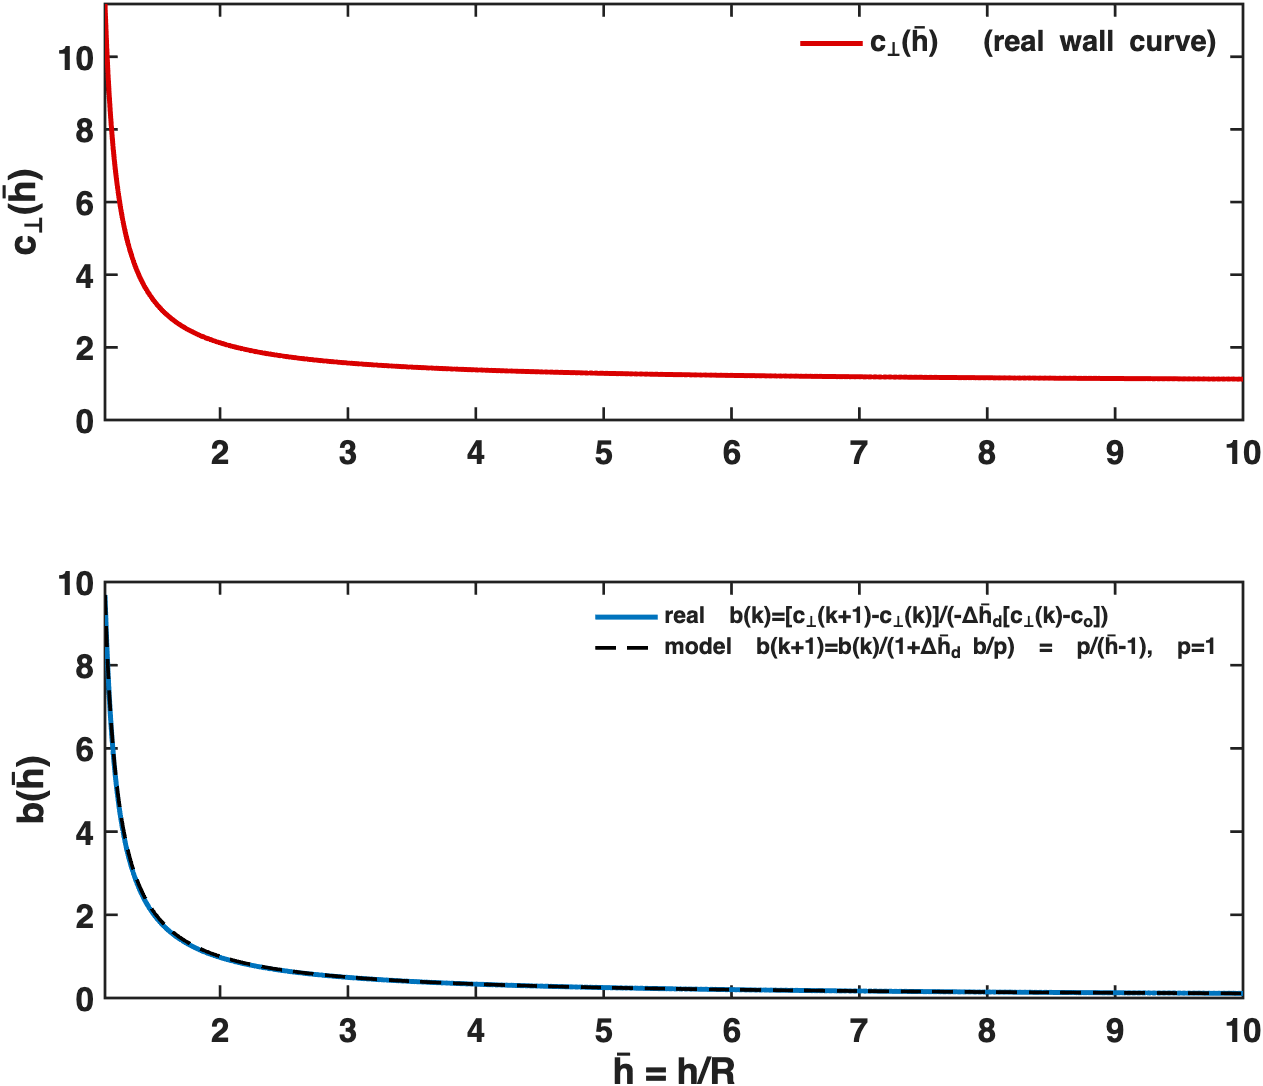
\includegraphics[width=0.94\linewidth]{figures/blocal_exp_check.png}
\end{center}

\newpage
\begin{center}
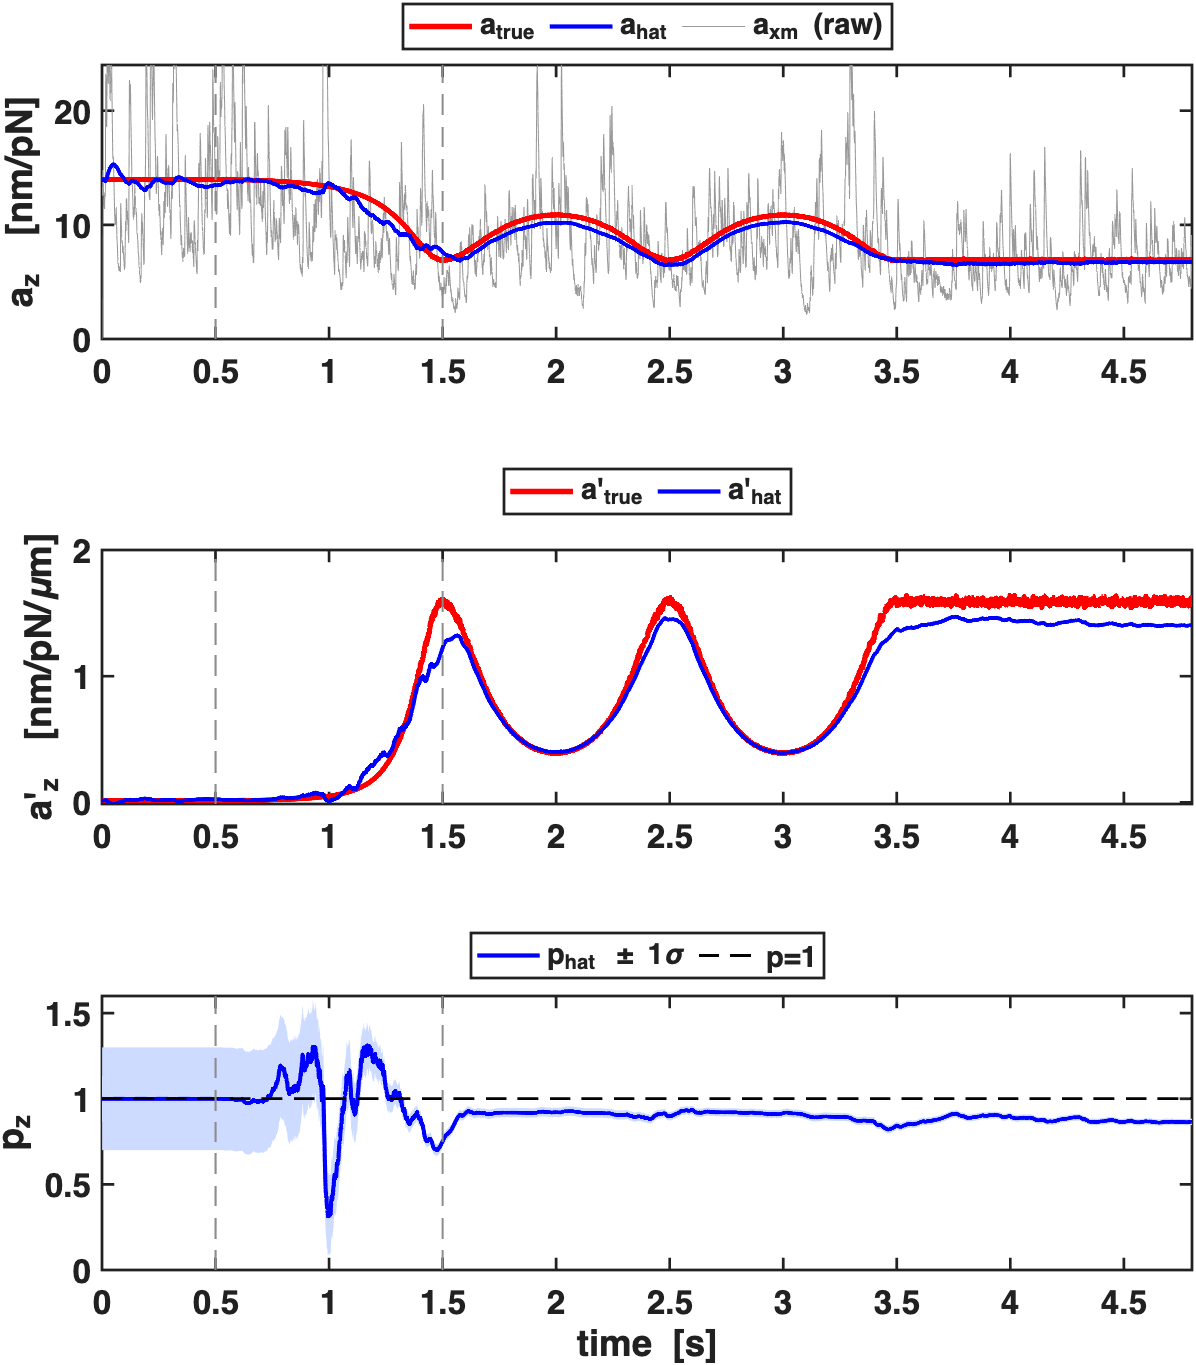
\includegraphics[width=0.66\linewidth]{figures/powerlaw_5state_sim.png}
\end{center}

\end{document}
